\chapter{计算机立体视觉基础}
\label{cha:chapVSLAM}
\section{引言}
\label{sec:chapVSLAM.1}
引言引言
\section{图像处理}
\section{相机模型}
相机能够将三维世界中的坐标点映射到二维图像平面中,这个过程可以利用数学建立几何模型进行描述,此类模型有很多种, SLAM中最常用的模
型为针孔模型。该模型描述了一束光通过针孔后,在针孔背面投影成像的关系,再同时考虑透镜的存在,会使得光线投影产生畸变,本文将利用针
孔和畸变两个模型来描述整个过程。
\subsection{刚体运动数学模型}
相机也可以看成三维空间中的刚体,即保证了同一个向量在各个坐标系下的长度和夹角都不会发生变化,因此需要考虑相机的位姿,即旋转和平移。
对于平移可以利用向量来表示,旋转则利用旋转矩阵,旋转向量,欧拉角,四元数等方式来描述,本文也将主要说明旋转过程的数学描述。

\textbf{旋转矩阵:}对于任意向量{~p~},在两个坐标系的描述为:
\begin{equation}
  \left[\mathbf{e}_{1}, \mathbf{e}_{2}, \mathbf{e}_{3}\right]\left[\begin{array}{l}{a_{1}} \\ {a_{2}} \\ {a_{3}}\end{array}\right]=\left[\mathbf{e}_{1}^{\prime}, \mathbf{e}_{2}^{\prime}, \mathbf{e}_{3}^{\prime}\right]\left[\begin{array}{c}{a_{1}^{\prime}} \\ {a_{2}^{\prime}} \\ {a_{3}^{\prime}}\end{array}\right]
\end{equation}

等式两边同时左乘$\left[\begin{array}{ccc}{\mathbf{e}_{1}^{T},} & {\mathbf{e}_{2}^{T},} & {\mathbf{e}_{3}^{T}}\end{array}\right]^{T}$可得
\begin{equation}
\left[\begin{array}{l}{a_{1}} \\ {a_{2}} \\ {a_{3}}\end{array}\right]=\left[\begin{array}{lll}{e_{1}^{T} e_{1}^{\prime}} & {e_{1}^{T} e_{2}^{\prime}} & {e_{1}^{T} e_{3}^{\prime}} \\ {e_{2}^{T} e_{1}^{\prime}} & {e_{2}^{T} e_{2}^{\prime}} & {e_{2}^{T} e_{3}^{\prime}} \\ {e_{3}^{T} e_{1}^{\prime}} & {e_{3}^{T} e_{2}^{\prime}} & {e_{3}^{T} e_{3}^{\prime}}\end{array}\right]\left[\begin{array}{c}{a_{1}^{\prime}} \\ {a_{2}^{\prime}} \\ {a_{3} ;}\end{array}\right]=\mathbf{R a}^{\prime}
\end{equation}

对于旋转矩阵R,即可描述旋转过程,并且R可以定义为特殊正交群:
\begin{equation}
  S O(n)=\left\{\mathbf{R} \in R^{n \times n} | \mathbf{R} \mathbf{R}^{T}=\mathbf{I}, \operatorname{det}(\mathbf{R})=1\right\}
\end{equation}

\textbf{旋转向量:}旋转矩阵在描述旋转时存在参数冗余和自身约束的问题,因此提出一个更加紧凑的数学描述$\theta_{n}$,旋转向量方向为旋转轴{~n~},
大小为旋转角$\theta$。旋转向量和旋转矩阵的转换可以用罗德里格斯公式表示:
\begin{equation}
  \mathbf{R}=\cos \theta \mathbf{I}+(1-\cos \theta) \mathbf{n} \mathbf{n}^{T}+\sin \theta \mathbf{n}^{\wedge}
\end{equation}

反之则有
\begin{equation}
  \operatorname{tr}(\mathbf{R})=\cos \theta \operatorname{tr}(\mathbf{I})+(1-\cos \theta) \operatorname{tr}\left(\mathbf{n} \mathbf{n}^{T}\right)+\sin \theta \operatorname{tr}\left(\mathbf{n}^{\wedge}\right)=1+2 \cos \theta
\end{equation}

\textbf{欧拉角:}将旋转运动分解成分别绕三个坐标轴的旋转($[r, p, y]^{T}$)来表示的,三个旋转的总和即为总的旋转,表述最为直观。

\textbf{四元数:}由于欧拉角和旋转向量存在奇异性,且不存在不带奇异性的三维向量描述方式,因此提出四元数这种紧凑且没有奇异性的数学
描述。四元数可以描述为:
\begin{equation}
  \mathbf{q}=q_{0}+q_{1} i+q_{2} j+q_{3} k=\{s, \mathbf{v}\}
\end{equation}
可以用单位四元数来描述空间中的任意旋转,假设旋转的描述为$\theta_{n}$,则:
\begin{equation}
  \mathbf{q}=\left[\cos \frac{\theta}{2}, n_{x} \sin \frac{\theta}{2}, n_{y} \sin \frac{\theta}{2}, n_{z} \sin \frac{\theta}{2}\right]^{T}
\end{equation}
旋转描述为R时,则:
\begin{equation}
\mathbf{R}=\left[\begin{array}{ccc}{1-2 q_{2}^{2}-2 q_{3}^{2}} & {2 q_{1} q_{2}-2 q_{0} q_{3}} & {2 q_{1} q_{3}+2 q_{0} q_{2}} \\ {2 q_{1} q_{2}+2 q_{0} q_{3}} & {1-2 q_{1}^{2}-2 q_{3}^{2}} & {2 q_{2} q_{3}-2 q_{0} q_{1}} \\ {2 q_{1} q_{3}-2 q_{0} q_{2}} & {2 q_{2} q_{3}+2 q_{0} q_{1}} & {1-2 q_{1}^{2}-2 q_{2}^{2}}\end{array}\right]
\end{equation}
反之则有:
\begin{equation}
  q_{0}=\frac{\sqrt{\operatorname{tr}(\mathbf{R})+1}}{2}, q_{1}=\frac{m_{23}-m_{32}}{4 q_{0}}, q_{2}=\frac{m_{31}-m_{13}}{4 q_{0}}, q 3=\frac{m_{12}-m_{21}}{4 q_{0}}
\end{equation}
通过以上方式都可以描述刚性运动中的旋转过程R,结合物体的平移t,则变化后的坐标为:
\begin{equation}
  \mathbf{a}^{\prime}=\mathbf{R} \mathbf{a}+\mathbf{t}
\end{equation}

在实际的使用中,由于以上等式非线性,可以引入齐次坐标T,可以将上式改成:
\begin{equation}
\left[\begin{array}{l}{\mathbf{a}^{\prime}} \\ {1}\end{array}\right]=\left[\begin{array}{ll}{\mathbf{R}} & {\mathbf{t}} \\ {\mathbf{0}^{T}} & {1}\end{array}\right]\left[\begin{array}{l}{\mathbf{a}^{\prime}} \\ {1}\end{array}\right]=\mathbf{T}\left[\begin{array}{l}{\mathbf{a}} \\ {1}\end{array}\right]
\end{equation}

对于变换矩阵T,可以定义为特殊欧氏群:
\begin{equation}
S E(3)=\left\{T=\left[\begin{array}{cc}{\mathbf{R}} & {\mathbf{t}} \\ {\mathbf{0}^{T}} & {1}\end{array}\right] \in R^{4 \times 4} | \mathbf{R} \in S O(3), t \in R^{3}\right\}
\end{equation}




\subsection{针孔相机模型}
对于针孔相机模型,如图~\ref{fig:2VSLAM_pinehole}所示,(其中f为相机焦距)存在4个坐标系分别为:世界坐标系,相机坐标系,图像坐
标系和像素坐标系,对于真实世界中的空间点$P_w$($X_w$,$Y_w$,$Z_w$),其对应的相机坐标系坐标为$P_c$($C_w$,$C_w$,$C_w$),
对应的图像坐标系为$P^{'}$($X^{'}$,$Y^{'}$),对应的像素坐标系为p(u,v)。
\begin{figure}[H] % use float package if you want it here
  \centering
  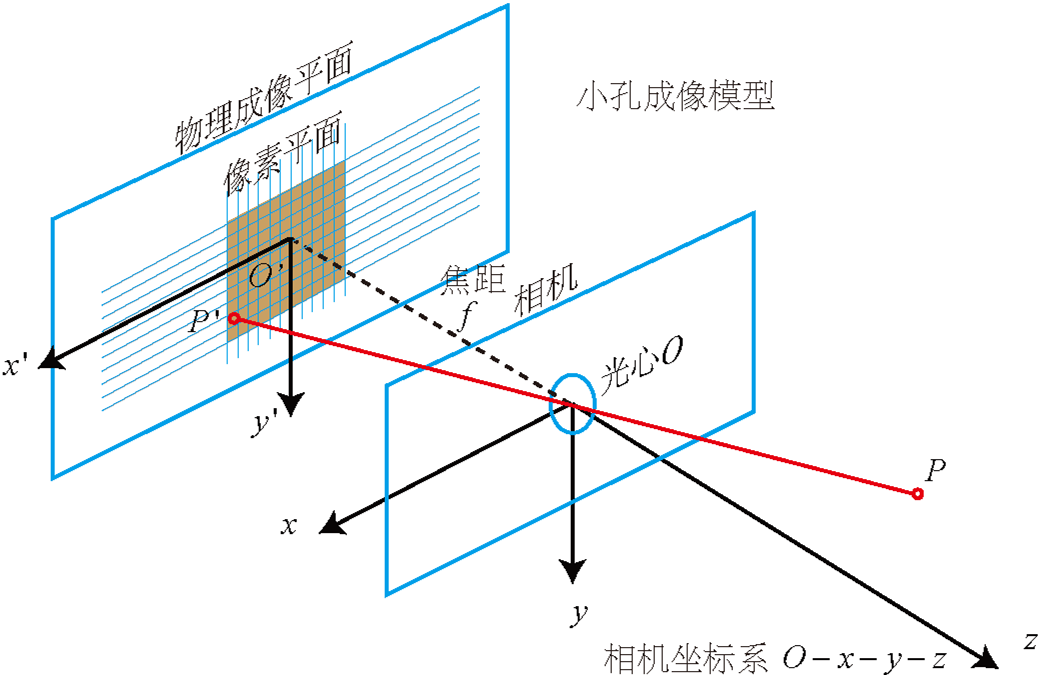
\includegraphics[height=6cm]{2VSLAM_pinehole.png}
  \caption{针孔相机模型}
  \label{fig:2VSLAM_pinehole}
\end{figure}
对于世界坐标系到相机坐标系之间的转化:
\begin{equation}
  \left[\begin{array}{l}{X c} \\ {Y_{C}} \\ {Z_{C}}\end{array}\right]=R\left[\begin{array}{l}{X w} \\ {Y w} \\ {Z w}\end{array}\right]+t
  \label{equ:world2cam}
\end{equation}
对于相机坐标系到图像坐标系之间的转化,可以利用如图~\ref{fig:2VSLAM_similartri}所示的相似三角形来求解:
\begin{equation}
  \begin{split}
    \frac{Z c}{f}=\frac{X c}{X^{'}}=\frac{Y c}{Y^{'}}\\
    \left\{\begin{array}{l}{X^{\prime}=f \frac{X c}{Z c}} \\ {Y^{\prime}=f \frac{Y c}{Z c}}\end{array}\right.
\end{split}
\label{equ:cam2photo}
\end{equation}
对于图像坐标系到像素坐标系的转化,如图~\ref{fig:2VSLAM_pixeltrans}所示:
\begin{equation}
  \begin{split}
    \left\{\begin{array}{l}{u=\frac{X^{\prime}}{d_{x}}+u_{o}} \\ {v=\frac{Y^{\prime}}{d_{y}}+v_{o}}\end{array}\right.\\
    \left[\begin{array}{l}{u} \\ {v} \\ {1}\end{array}\right]=\left[\begin{array}{ccc}{\frac{1}{d_{x}}} & {0} & {u_{o}} \\ {0} & {\frac{1}{d_{x}}} & {v_{o}} \\ {0} & {0} & {1}\end{array}\right]\left[\begin{array}{c}{X^{\prime}} \\ {Y^{\prime}} \\ {1}\end{array}\right]
  \end{split}
  \label{equ:photo2pixel}
\end{equation}
\begin{figure}[H]
  \centering%
  \subcaptionbox{相机坐标系到图像坐标系转换\label{fig:2VSLAM_similartri}}{%    
    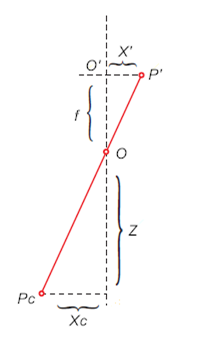
\includegraphics[height=4cm]{2VSLAM_similartri.png}}\hspace{6em}%
  \subcaptionbox{图像坐标系到像素坐标系转换\label{fig:2VSLAM_pixeltrans}}{%    
    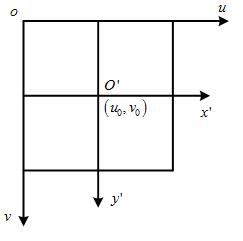
\includegraphics[height=4cm]{2VSLAM_pixeltrans.png}}
  \caption{坐标系转化示意图}
  \label{fig:trans}
\end{figure}
其中$d_x$,$d_y$分别表示沿着x,y轴的实际物理尺寸,($u_o$,$v_o$)表示光心对应到像素坐标系得到坐标.由公式~\ref{equ:cam2photo}和
~\ref{equ:photo2pixel}可以转化得到相机坐标系到像素坐标系的关系:
\begin{equation}
Z c\left[\begin{array}{l}{u} \\ {v} \\ {1}\end{array}\right]=\left[\begin{array}{ccc}{\frac{f}{d_{x}}} & {0} & {u_{0}} \\ {0} & {\frac{f}{d_{y}}} & {v_{0}} \\ {0} & {0} & {1}\end{array}\right]\left[\begin{array}{c}{X_{c}} \\ {Y_{c}} \\ {Z_{c}}\end{array}\right]=\left[\begin{array}{ccc}{f_{x}} & {0} & {u_{0}} \\ {0} & {f_{y}} & {v_{0}} \\ {0} & {0} & {1}\end{array}\right]\left[\begin{array}{c}{X_{c}} \\ {Y_{c}} \\ {Z_{c}}\end{array}\right]=K\left[\begin{array}{c}{X_{c}} \\ {Y_{c}} \\ {Z_{c}}\end{array}\right]
  \label{equ:cam2pixel}
\end{equation}
由公式~\ref{equ:world2cam}和~\ref{equ:cam2pixel}得到世界坐标系到像素坐标系的转化关系为:
\begin{equation}
Z c\left[\begin{array}{l}{u} \\ {v} \\ {1}\end{array}\right]=K(R P w+t)=K\left(R\left[\begin{array}{l}{X w} \\ {Y w} \\ {Z w}\end{array}\right]+t\right)
\end{equation}
其中K表示相机内参矩阵,R,t表示相机外参。


\subsection{相机畸变模型}
为了使得相机产生更好的成像效果,会加入透镜,透镜的加入对成像过程中光线的传播产生影响会引入径向畸变,这类畸变可以用于距中心的距离
有关的二次及高次多项式函数进行修正。
\begin{equation}
\left\{\begin{array}{l}{x_{r a d}=x\left(1+k_{1} r^{2}+k_{2} r^{4}+k_{3} r^{6}\right)} \\ {y_{r a d}=y\left(1+k_{1} r^{2}+k_{2} r^{4}+k_{3} r^{6}\right)}\end{array}\right.
\end{equation}

在相机的组装过程中,由于不可能保证透镜和相机得到成像平面得到的完全平行,也会引入切向畸变,可以使用两个参数$p_1$,$p_2$来进行修
正。
\begin{equation}
  \left\{\begin{array}{l}{x_{\tan }=x+2 p_{1} x y+p_{2}\left(r^{2}+2 x^{2}\right)} \\ {y_{\tan }=y+p_{1}\left(r^{2}+2 y^{2}\right)+2 p_{2} \pi y}\end{array}\right.
\end{equation}

联合公式,对于相机坐标系中的点P(X,Y,Z),通过以上5个畸变参数找到该点在像素坐标系上的正确位置。
\begin{equation}
  \left\{\begin{array}{l}{x_{\text {corrected}}=x\left(1+k_{1} r^{2}+k_{2} r^{4}+k_{3} r^{6}\right)+2 p_{1} \pi y+p_{2}\left(r^{2}+2 x^{2}\right)} \\ {y_{\text {corrected}}=y\left(1+k_{1} r^{2}+k_{2} r^{4}+k_{3} r^{6}\right)+p_{1}\left(r^{2}+2 y^{2}\right)+2 p_{2} x y}\end{array}\right.
\end{equation}


\section{SLAM框架}
SLAM(simultaneous Localization and Mapping)是指同时的定位和地图构建,依靠特定的传感器在没有环境先验知识信息的情况下,在运
动的过程中建立环境的模型。当传感器为相机时,则称之为视觉SLAM,本文也将主要讨论视觉SLAM的主要流程框架,主要包括特征提取,特征点
匹配,视觉里程计,跟踪过程,建图和后端优化等。
\subsection{特征提取}
特征是图像信息的另外一种数字表现形式,良好的特征应该是不受光线,噪音,几何变形影响的。特征提取的目的是为了后续能够尽可能准确、稳
定地估计出相机的运动,特征点能够具备可重复性,高效率,可区别性以及本地性的特点,经过几十年的发展,在图像处理领域已经提出了多种特
征提取的方法。

\textbf{Harris角点:}当从不同的方向去移动一个视觉窗口,假设该区域内的灰度发生了很大的的变化,则认定存在角点。对于图像I(x,y),
当在点(x,y)处平移(Δx,Δy)后的对应窗口的像素点灰度变化描述为:
\begin{equation}
  c(x, y ; \Delta x, \Delta y)=\sum_{(u, v) \in W(x, y)} (I(u, v)-I(u+\Delta x, v+\Delta y))^{2}
  \label{equ:Harris}
\end{equation}
结合泰勒分解公式,上式可以化简为:
\begin{equation}
  c(x, y ; \Delta x, \Delta y) \approx \sum_{w}\left(I_{x}(u, v) \Delta x+I_{y}(u, v) \Delta y\right)^{2}=[\Delta x, \Delta y] M(x, y)\left[\begin{array}{c}{\Delta x} \\ {\Delta y}\end{array}\right]
\end{equation}
其中
\begin{equation}
  \begin{split}
   & M(x, y)=\sum_{w}\left[\begin{array}{cc}{I_{x}(x, y)^{2}} & {I_{x}(x, y) I_{y}(x, y)} \\ {I_{x}(x, y) I_{y}(x, y)} & {I_{y}(x, y)^{2}}\end{array}\right]\\
   & =\left[\begin{array}{cc}{\sum_{w} I_{x}(x, y)^{2}} & {\sum_{w} I_{x}(x, y) I_{y}(x, y)} \\ {\sum_{w} I_{x}(x, y) I_{y}(x, y)} & {\sum_{w} I_{y}(x, y)^{2}}\end{array}\right] \\
   & =\left[\begin{array}{cc}{A} & {C} \\ {C} & {B}\end{array}\right] 
  \end{split}
  \end{equation}
公式~\ref{equ:Harris}即可转化为
\begin{equation}
  c(x, y ; \Delta x, \Delta y) \approx A \Delta x^{2}+2 C \Delta x \Delta y+B \Delta y^{2}
\end{equation}
又提出角度响应值R来判断该点是否为角点:
\begin{equation}
  R=\operatorname{det} \boldsymbol{M}-\alpha(\operatorname{trace} \boldsymbol{M})^{2}
\end{equation}
通过以上公式可以看出,Harris角点具备以下特点:\\
1. 对亮度和对比度的变化不敏感:因为微分运算对图像密度的变化不敏感,即亮度或者对比度的变化对Harris的检出影响较小;\\
2. 具有旋转不变性:Harris角点检测算子的本质可以表示为一个椭圆,但椭圆旋转时,并不会影响R值的大小;\\
3. 不具有尺度不变性。

\textbf{FAST特征点:}对图像中的中的一个像素p,假设其亮度值为$I_p$,阈值为t,如图所示,取以其为中心,半径为是三个像素的圆,
圆上共有16个像素点,假设这16个点中有连续N个点都比$I_p+t$大或者比$I_p-t$小,则认定其为Fast角点,为了加快检测过程,会直接检
测第1,5,9,13这4个点,如果有三个满足要求,也会认为是角点。
\begin{figure}[H] % use float package if you want it here
  \centering
  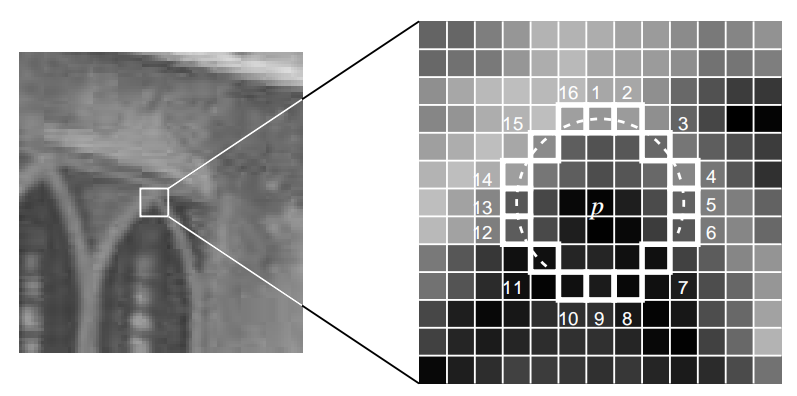
\includegraphics[height=6cm]{2VSLAM_Fast.png}
  \caption{FAST特征点}
  \label{fig:2VSLAM_Fast}
\end{figure}
\textbf{ORB特征点:}结合了FAST特征点的检测和BRIEF描述子,其中RIEF特征描述符的计算过程:首先平滑图像,在某个像素点的周围选
择一个领域,根据特定的点对选择方法挑选出$n_d$个点对,比较每个点对之间亮度值的大小,即可得到一个长度为$n_d$的二进制串。
由于FAST特征点不具有方向,ORB在此基础上进行了改良,即利用灰度质心法求解出灰度额质心之间的偏移方向,首先定义特征点p的邻域像素的矩:
\begin{equation}
  m_{p q}=\sum_{x, y} x^{p} y^{q} I(x, y)
\end{equation}
图像的质心为:
\begin{equation}
  C=\left(\frac{m_{10}}{m_{00}}, \frac{m_{01}}{m_{00}}\right)
\end{equation}
那么偏移方向可以定义为FAST的特征点方向:
\begin{equation}
  \theta=\arctan \left(m_{01}, m_{10}\right)
\end{equation}
通过以上内容说明了SLAM框架中常用的特征点提取方式,接下来将以此为基础说明特征点的匹配过程:即在已知参考帧和当前参考帧的特征点
信息时,求解这两帧中相同的特征点。计算两帧中的汉明距离是常用的特征匹配方法,即计算两个等长描述符对应位置上不同数字的个数,数
值越小,越相似。如图~\ref{fig:2VSLAM_ORB_match}所示为通过提取ORB特征进行匹配的结果。
\begin{figure}[H] % use float package if you want it here
  \centering
  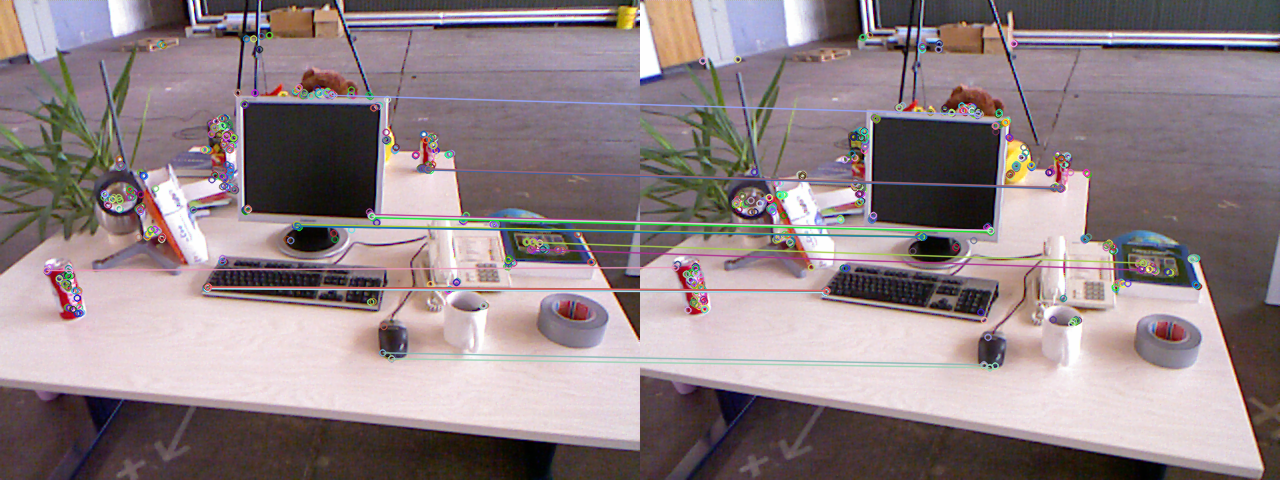
\includegraphics[height=6cm]{2VSLAM_ORB_match.png}
  \caption{ORB特征匹配结果}
  \label{fig:2VSLAM_ORB_match}
\end{figure}



\subsection{视觉里程计}
视觉里程计是指通过相机提供得到连续图像信息来估计相邻帧之间得到相机运动情况,将所有的相对运动都转化为以第一帧为参考的位姿信息。在
整个视觉里程计的计算过程中,需要通过上一节的特征点匹配来完成初始化,视觉SLAM初始化时,会分别计算单应矩阵和基础矩阵。
\begin{figure}[h] % use float package if you want it here
  \centering
  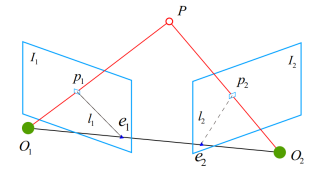
\includegraphics[height=6cm]{2VSLAM_Epipolar_Geometry.png}
  \caption{对极约束模型}
  \label{fig:2VSLAM_Epipolar_Geometry}
\end{figure}
首先需要说明对极约束,其描述了图像中特征点位置和帧之间运动情况之间的关联,如图~\ref{fig:2VSLAM_Epipolar_Geometry}所示,
假设$I_1$和$I_2$为相邻帧,$p_1$和$p_2$为相邻帧中的对应特征点,P为空间中实际的特征点,R,t为两帧之间的运动变化。通过对极约
束可以得到:
\begin{equation}
  p_{2}^{T} K^{-T} t^{\wedge} R K^{-1} p_{1}=0
\end{equation}
其中定义本质矩阵$ E = t^{\wedge} R$,基础矩阵$F =  K^{-T}E K^{-1}$,以上特征点的匹配可以解出E,再利用奇异值分解可以恢复出
相机的运动R,t。

对于单应矩阵,描述的是两个平面之间的映射关系,通常用于特征点都落在同一片面内的条件下,通过非奇异性矩阵H就可以实现两张图之间的
变化,单应矩阵可以用于纯旋转的条件下。$(u_1,v_1,1)^{T}$,$(u_2,v_2,1)^{T}$分别是两张图像中的像素点,变化形式:
\begin{equation}
\left(\begin{array}{l}{u_{1}} \\ {v_{1}} \\ {1}\end{array}\right)=\left(\begin{array}{lll}{h_{11}} & {h_{12}} & {h_{13}} \\ {h_{21}} & {h_{22}} & {h_{23}} \\ {h_{31}} & {h_{32}} & {h_{33}}\end{array}\right)\left(\begin{array}{l}{u_{2}} \\ {v_{2}} \\ {1}\end{array}\right)
\end{equation}
假设平面π在第一个相机坐标系下的单位法向量为$n_T$,距离相机光心的距离为d,则平面$\pi$可以表示为:
\begin{equation}
  n^{T} X_{1}=d
\end{equation}
$X_1$,$X_2$分别三维点P在两台相机坐标系下的坐标,则有:
\begin{equation}
  \begin{split}
    X_{2} &=R X_{1}+t \\ 
    X_{2}=R X_{1}+t \frac{1}{d} n^{T} X_{1} &=\left(R+t \frac{1}{d} n^{T}\right) X_{1}=H X_{1} \\ 
    H &=R+t \frac{1}{d} n^{T} 
  \end{split}
\end{equation}
假设$p_1$,$p_2$分别为$X_1$,$X_2$对应的图像上的点,则:
\begin{equation}
\begin{aligned} X_{1} &=K^{-1} p_{1}, X_{2}=K^{-2} p_{1} \\ H &=K\left(R+t \frac{1}{d} n^{T}\right) K^{-1} \end{aligned}
\end{equation}
通过以上过程,可以发现SLAM的初始化要求前后帧之间有足够的视差,并且不能只是纯旋转运动,对于求解出来的t也是没有明确物理尺度的。
\subsection{追踪}
在初始化成功后,对于相机获取的当前图像,可以通过追踪匹配到上一帧特征点的方式来获取相机位姿得到初始值,在追踪流程中,一般会兼顾
利用到一下三种模型三种模型:\\
\textbf{运动模型:}根据两帧之间的约束关系来解算相机的位姿,这一模型是建立在物体匀速运行的假设上,可以利用上一帧的位姿来估算当前帧的位姿。如果物体静止或者运动模式失效,则可以增加参考帧的地图点反投影匹配范围,获得更多的匹配来计算当前位姿。\\
\textbf{关键帧模式:}如果上种模式失效,则首先尝试和最近一个关键帧去做匹配,计算当前帧的词袋模型,以上一帧的位姿作为当前帧的位姿,在根据位姿和磁带模型寻找特征匹配以优化位姿。\\
\textbf{重定位模式:}如果上述两种追踪模型都失效,则整个SLAM处于丢失状态,此时就需要通过重定位俩重新追踪。重定位的流程:\\
1.	计算当前帧的BoW向量\\
2.	依靠BoW词典,在关键帧集合中寻找到与当前帧相似的候选匹配帧\\
3.	通过BoW匹配当前帧和每一个候选关键帧,通过PnP求解位姿\\
4.	对以上位姿进行BA优化,当内点数量超过某一阈值时,则保留该关键帧,并通过反投影获取额外的地图点加入优化。\\
